\documentclass{report}
% 导言区
\usepackage{xeCJK}
\usepackage{graphicx}
\graphicspath{{figures/}}
\usepackage{float}
\usepackage{amsmath}
% 加深编号
\setcounter{secnumdepth}{3}
% 标题信息
\title{移动通信}
\author{张兴锐}
\date{2018-3-25}
\begin{document}
	\maketitle
	\tableofcontents
	% 
	\chapter{概论}
	\section{移动通信特点}
	\subsection{什么是移动通信?}
	\textbf{定义:}移动通信就是通信双方至少有一方是处于运动中进行信息交换的通信方式。其移动性包括:
	\begin{itemize}
		\item 终端的移动性,特定的“终端号码(如手机串号,\verb|*#06#| )“,手机,车载台
		\item 个人的移动性,特定的”个人号码,SIM卡号”。
	\end{itemize}
	\subsection{移动通信特点}
	\begin{enumerate}
		\item 移动通信必须利用无线电波进行信息传输。
		\begin{enumerate}
			\item 弥散损耗(自由传播损耗),随着传播距离的增加而损耗。
			\item 阴影效应,受到地形、地物的遮蔽而发生。
			\item 多径效应,信号经过多点反射,会从多条路径到达接受地点,这种多径信号的\textbf{幅度、相位和到达时间}都不一样,它们会叠加而产生“多径效应”。
			\item 多普勒-效应
		\end{enumerate}
		\item 移动通信是在复杂的干扰环境中运行的。
		\begin{enumerate}
			\item 外部干扰。天电干扰、工业干扰和信道噪声
			
			\item 系统间干扰。
			\begin{enumerate}
				\item 邻道干扰
				\item 互调干扰(当两个或多个干扰信号同时加到接收机时,\textbf{由于非线性的作用},这两个干扰的组合频率有时会恰好等于或接近有用信号频率而顺利通过接收机,这种干扰就称为互调干扰,其中三阶互调最严重。)
				\item 同频道
				干扰(蜂窝移动通信)
				\item 多址干扰(多址干扰是指同\textbf{CDMA}系统中多个用户的信号在时域和频域上是混叠的。因为\textbf{CDMA}系统为码分多址,CDMA系统采用的是不同的地址码来区分每个用户,但多个用户的信号在时域和频域上是混叠的,所以在频域在产生一定的同频和邻频干扰,则为多址干扰。)
				\item 远近效应
			\end{enumerate}
			
			\item 抗干扰技术。扩频技术、信道编码与交织技
			术、信道均衡技术、分集技术、信道估计技
			术、信号检测技术和智能天线技术
			
		\end{enumerate}
		\item 移动通信业务量的需求与日俱增,而频率资源
		非常有限。
		\item 移动通信系统的网络结构多种多样,网络管
		理和控制必须有效。
		\item 移动通信设备必须适于在移动环境中满足多种应
		用要求。
	\end{enumerate}
	\section{常用移动通信系统}
	\begin{enumerate}
		\item  公共陆地移动通信网络(PLMN)
		\item 无线市话系统(WUTS)
		\item 集群系统(专网)--->公安系统,水利系统、交通系统、电力系统、铁路系统。
		\item 卫星移动通信系统。
		\item 无线局域网。
	\end{enumerate}
	\section{移动通信系统发展}
	\begin{figure}[H]
		\centering
		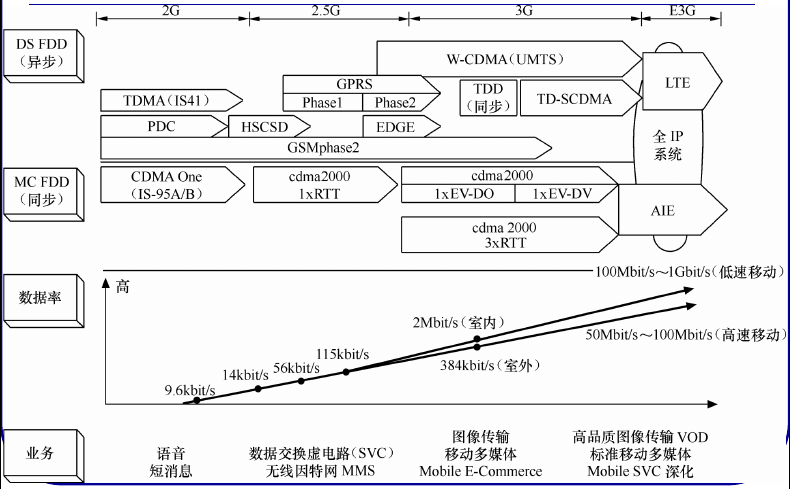
\includegraphics[scale=0.7]{移动通信系统2G_4G发展.png}
		\caption{移动通信系统发展}
	\end{figure}
	\begin{figure}[H]
		\centering
		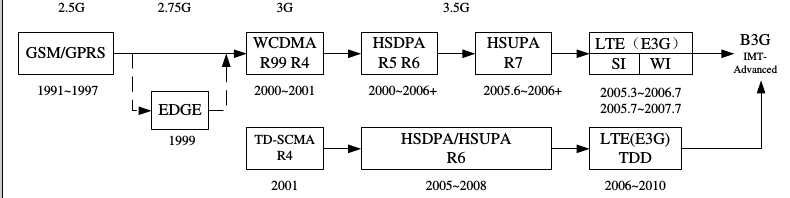
\includegraphics[scale=0.7]{WCDMA_TD-SCDMA发展.png}
		\caption{WCDMA\&TD-SCDMA发展}
	\end{figure}
	\begin{figure}
		\centering
		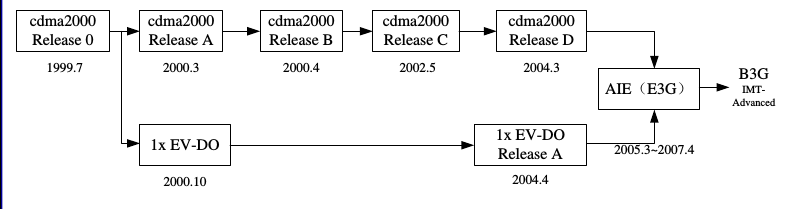
\includegraphics[scale=0.7]{CDMA2000发展.png}
		\caption{CDMA2000发展}
	\end{figure}
	\section{蜂窝移动通信的组网技术}
	\subsection{多址接入}
	\subsubsection{什么是多址接入?}
	\textbf{定义:}移动通信系统中,使所有的用户共享
	有限的无线资源,实现不同用户不同地点同时
	通信,并尽可能减少干扰。
	\subsubsection{多路复用和多址接入区别}
	\textbf{相同点:}两者的理论基础都是\textbf{信号的正交分割原理。}
	
	\textbf{不同点:}
	\begin{itemize}
		\item \textbf{”点对点“},多路复用
		\item \textbf{"点多多点"},多址接入
	\end{itemize}
	
	\subsubsection{多址接入分类}
	\begin{enumerate}
		\item 频分多址: 第一代移动通信系统;TACS、AMPS。
		\item 时分多址: 第二代移动通信系统:GSM。
		\item 码分多址: 第三代移动通信系统:IS-95 CDMA、WCDMA。存在两个重要问题:
		\begin{enumerate}
			\item  多址干扰
			\item  远近效应.
		\end{enumerate}
		\item 空分多址。
		\item OFDMA.正交频分多址
		\item NOMA,非正交频分多址
	\end{enumerate}
	\subsection{工作方式}
	\begin{enumerate}
		\item 单工::通信双方电台交替地进行收信和
		发信。\textbf{对讲机}。
		\item 半双工:是指通信双方中,一方使用双
		频双工方式,即收发信机同时工作;另一
		方使用双频单工方式,即收发信机交替工
		作。\textbf{基站-手机}。基站处于全双工,手机处于半双工。
		\item 全双工:是指通信双方收发信机均同时工
		作。收信和发信必须\textbf{采用不同的工作频率},\textbf{打电话}	\\
		
		双工模式:
		\begin{enumerate}
		\item 频分双工FDD。
		\item 时分双工TDD。
		\end{enumerate}
		两种模式的区别:
		\begin{itemize}
			\item 由于TDD方式的时间资源\textbf{分别分给了上行和下行,
			因此TDD方式的发射时间大约只有FDD的一半},如果
			TDD要发送和FDD同样多的数据,就要\textbf{增大TDD的发
			送功率。}
			\item TDD可以通过调整上下行时隙转换点,改变上下行
			时隙比例,可\textbf{很好地支持非对称业务}。
			\item TDD系统上行受限,因此TDD基站的\textbf{覆盖范围明显小}
			于FDD基站。
			\item FDD模式的特点是在分离(上下行频率间隔45MHz、
			190MHz等)的两个对称频率信道上,系统进行接收
			和传送,用保护频段来分离接收和传送信道。相当
			于分道行驶,比较顺畅,所以\textbf{FDD速度会更快}。
			
		\end{itemize}
%		\hspace{-5em}
		\begin{center}
			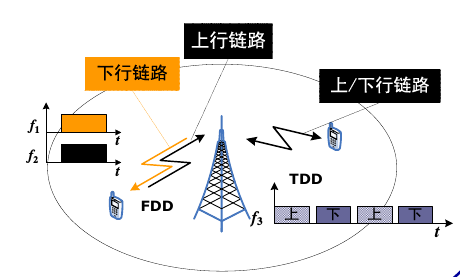
\includegraphics[scale=1]{双工模式.png}
		\end{center}
	\end{enumerate}
	\subsection{频率复用和蜂窝小区}
	\subsubsection{移动通信网的区域覆盖方式}
	\begin{enumerate}
		\item 小容量的大区制(发射功率大)
		\item  大容量的小区制,(频率复用)
	\end{enumerate}
	\subsubsection{区群}
	 \textbf{定义:}共同使用全部可用频率的N个小区组成一个区群。\\
	 \textbf{特点:}
	 \begin{enumerate}
	 	\item 同一个小区,使用不同的频率。
	 	\item 不同小区,可以使用相同频率。
	 \end{enumerate}
 	\textbf{组成区群的小区数对应的公式}:
 	\begin{eqnarray}
 		N = i^2+ij+j^2
 	\end{eqnarray}
	一个共有S个信道的蜂窝系统(一个区群),每簇含有N个小区(一个区群),每个小区含有K个信道。则:
	\begin{eqnarray}
		S = KN
	\end{eqnarray}
	将这个簇重复M次,则信道总数为C:
	\begin{eqnarray}
	C = MS = MKN
	\end{eqnarray}
	\subsubsection{同频道距离}
	\textbf{STEPS:}
	\begin{enumerate}
		\item 首先垂直六边形的任一边延长$Max{i,j}$个小区。
		\item 逆时针旋转60°,在延长$Min{i,j}$个小区。
	\end{enumerate}

	\begin{figure}[H]
		\centering
		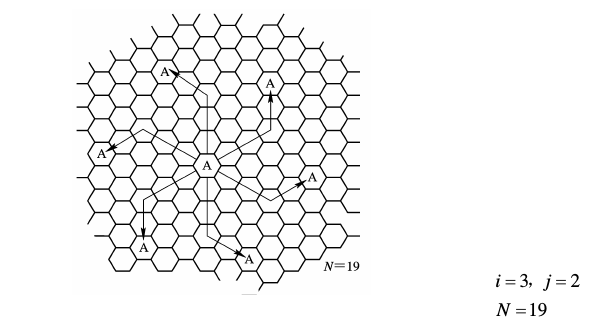
\includegraphics[scale=0.65]{通频道距离确定.png}
		\caption{通频道距离确定}
	\end{figure}
	\begin{minipage}[c]{0.8\linewidth}
			\begin{gather*}
		D^2 = I^2 + J^2 - 2IJ\cos120°	\\
		H = \frac{\sqrt{3}}{2}R	\\
		I = \sqrt{3}iR,J = \sqrt{3}jR	\\
		\Rightarrow 
		D = \sqrt{3N}R,\text{其中}N = i^2+ij+j^2
		\end{gather*} 
	\end{minipage}
	\begin{minipage}[r]{0.2\linewidth}
		\stepcounter{equation}
		(\theequation)
	\end{minipage}
	
	\subsubsection{同频干扰}
	移动台的接收载波干扰比为: \\

	\begin{gather}
		\frac{C}{I} = \frac{C}{\sum_{i=1}^{L}I_i} \notag  \\
		\frac{C}{I} = \frac{(D/R)^n}{L}=\frac{\sqrt{3N}^n}{L} 
		\label{eq:载干比}
	\end{gather}

	\text{其中,L为同频干扰小区数} \\
	n常取4,用Q表示同频复用比例$Q = \frac{D}{R}$。
	\subsubsection{蜂窝系统容量}
	通常衡量
	系统容量的指标是每小区的可用信道数来度量:
	\begin{equation}
		n = \frac{B_t}{B_cN}
	\end{equation}
	\begin{itemize}
		\item $B_t$ 系统总带宽
		\item $B_c$ 单个小区占用的信道带宽
		\item $N$ 频率复用因子,利用\ref{eq:载干比}计算
	\end{itemize}
	\begin{description}
		\item[FDMA系统] 
		
		\begin{equation*}
			N = \sqrt{\frac{2}{3}\times \frac{C}{I}}
		\end{equation*}
		
		\begin{equation}
		n = \frac{B_t}{B_c\sqrt{\frac{2}{3}\times \frac{C}{I}}}
		\end{equation}
		\item [TDMA系统]
		\begin{gather}
			n = \frac{B_t}{B_c^{'}\sqrt{\frac{2}{3}\times \frac{C}{I}}} \notag \\
			B_c^{'} = \frac{B_c}{m}
		\end{gather}
		m是每一频道包含的时隙数。
		\item[CDMA系统] 
		\begin{equation}
		n = [1+\frac{W/R_b}{E_b/I_0}\times \frac{1}{d}]\times G F
		\end{equation}
	\end{description}
	\subsubsection{提高蜂窝系统容量的方法
	}
	\begin{enumerate}
		\item 	基站发射机位置
		\begin{enumerate}
			\item  中心激励小区:安置在小区的中心
			\item  顶点激励小区:安置在六边形3个间隔的顶点上 \\
			\begin{center}
			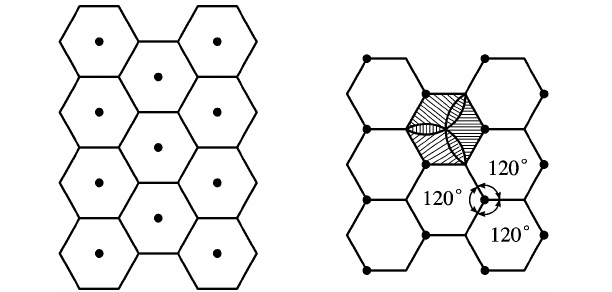
\includegraphics[scale=0.7]{基站发射机位置.png}
			\end{center}
		\end{enumerate}
		\item 小区分裂
		\item 划分扇区
		\item 新微小区
	\end{enumerate}
	\subsection{多信道共用技术}
	\begin{itemize}
		\item 信道 --> (1)控制信道,业务信道
		\item 信道共用
		\begin{center}
			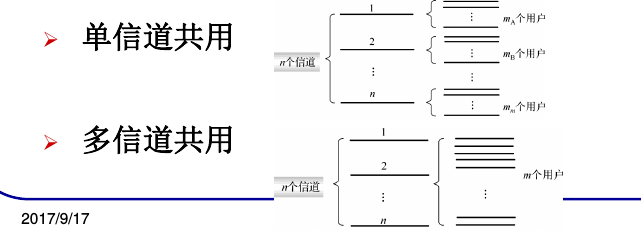
\includegraphics[width=\linewidth,height=4cm]{信道共用.png}
		\end{center}
	\end{itemize}
	话务理论的经典公式-爱尔兰呼损公式:
	\begin{equation}
	B = \frac{A^n/n}{\sum_{i=0}^{n}A^i/i!}
	\end{equation}
	其中
	\begin{itemize}
		\item B,呼损率
		\item A,流入话务量
		\item n,共用信道数
	\end{itemize}
	 信道利用率公式
	\begin{equation}
	\eta = \frac{A(1-B)}{n}
	\end{equation}
	用户忙时话务量:$\alpha = CTk\frac{1}{3600}$ \\
	每个共用信道所能容量的用户数:$m = \frac{A/n}{\alpha}$ \\
	n个共用信道所能容纳的总用户数:$N = mn = \frac{A}{\alpha}$
\end{document}